\documentclass[english, xcolor = {table}]{beamer}
\usepackage{slides_style}
\usepackage{dsfont}


%\usetikzlibrary{shapes.geometric,positioning}

\newcommand{\EoL}[1][2]{\lang{Eo}\text{-}{#1}\text{-}\lang{L}}


\title[Доказательства и вычисления]{
    Доказательства и монотонные вычисления
}

\author[Соколов Д.]{
    Дмитрий Соколов\\
    KTH University\\
    ПОМИ РАН\\
    \vspace{1cm}
    Ankit Garg, Mika G{\"{o}}{\"{o}}s,  Pritish Kamath, Robere Robert
}  


\date{МИАН-ПОМИ\\
	24 декабря\\
	2018
}


\begin{document}

    \maketitle

    \section{Part I: Dag Protocols and Lifting}

 %   \begin{frame}{Corollaries}
    $m = n^{O(1)}$, $w(\varphi)$ is the least width of resolution proof of $\varphi$

    \pause
    \begin{enumerate}
        \item \ba $\varphi$ the number of lines of any $\CP$ proof of $\varphi \circ \Ind_m$ is at least
            $n^{w(\varphi)}$.
        \pause
        \item \textbf{($\CP$ vs. $\NS$)} \be $\varphi$ such that:
            \begin{itemize}
                \item for any field $\mathbb{F}$ formula $\varphi$ has $\NS_{\mathbb{F}}$ proof of
                    $O(\log(n))$ degree;
                \item any $\CP$ proof of $\varphi$ has size at least $2^{n^{\varepsilon}}$ for some fixed
                    $\varepsilon > 0$.
            \end{itemize}
        \pause
        \vspace{0.4cm}    
        \item \ba $\varphi$ the size of any monotone circuit for $f_{\varphi \circ \Ind_m}$ is at least
            $n^{w(\varphi)}$ (\be $\varphi$ such that $f_{\varphi \circ \Ind_m} \in \NC^2$).
        \pause
        \item \be $f$ that can be computed by monotone span program of size $\poly(n)$ over any field,
            but any real monotone circuit for $f$ has size at least $2^{n^{\varepsilon}}$ for some fixed
            $\varepsilon > 0$.
    \end{enumerate}
\end{frame}

    \begin{frame}{Коммуникационные протоколы. $f: X \times Y \to \mathcal{O}$}
    \begin{center}
    	\onslide<1->{
    \tikzstyle{op1} = [opacity = 0]
    \tikzstyle{op2} = [opacity = 0]
    \tikzstyle{op3} = [opacity = 0]
    \tikzstyle{op4} = [opacity = 0]
}
\only<2->{\tikzstyle{op2} = [opacity = 1]}
\only<3->{\tikzstyle{op3} = [opacity = 1]}
\only<4->{\tikzstyle{op4} = [opacity = 1]}

\begin{tikzpicture}[>=latex]
    \node (alice) at (0, 0) {\includegraphics[scale = 0.15]{pics/utia-food-1.png}};
    \node (bob) at (7, 0) {\includegraphics[scale = 0.15]{pics/utia-food-2.png}};
    \node[above = 0.3 of alice] {$x \in U$};
    \node[above = 0.3 of bob] {$y \in V$};

    \path (alice.east) -- (bob.west) node[midway, above = 2.3] {\Large $f(x, y) = ?$};
    \draw[op2, ->, thick] ($(alice.east) + (0.3, 1)$) -- ($(bob.west) + (-0.3, 1)$) node[midway, above]
        {$r_1 = a(x)$};
    \draw[op3, <-, thick] ($(alice.east) + (0.3, 0.2)$) -- ($(bob.west) + (-0.3, 0.2)$)
        node[midway, above] {$r_2 = b(y, r_1)$};
    \draw[op4, ->, thick] ($(alice.east) + (0.3, -0.2)$) -- ($(bob.west) + (-0.3, -0.2)$);
    \draw[op4, ->, thick] ($(alice.east) + (0.3, -0.6)$) -- ($(bob.west) + (-0.3, -0.6)$)
        node[midway, below] {$\vdots$}; 
\end{tikzpicture}    
    \end{center}

    \pause
    \pause
    \pause
	\pause
    
    Глубина коммуникационного протокола~--- число раундов в худшем случае.
    
    $\CC(f)$~--- минимальная глубина коммуникационного прокола для функции $f$.
\end{frame}

\begin{frame}{Протоколы и деревья}

    Алиса получает $x \in X$, а Боб получает $y \in Y$. Коммуникационный протокол соответствует дереву:
    \begin{columns}[t]
		\begin{column}{0.7\textwidth}
            \begin{itemize}
                \item<2-> внутренние вершины помечены игроками;
	            \item<3-> текущий игрок посылает бит и игроки переходят в следующую вершину;
    		    \item<8-> листья помечены ответами.
	        \end{itemize}

    		\onslide<9->{
                Размер протокола~--- размер соответствующего дерева.
            } 
        \end{column}
        
		\begin{column}{0.25\textwidth}
            \tikzstyle{inner} = [thin, circle, minimum size = 0.3cm, draw, inner sep = 0.1pt, black]
\tikzstyle{gstyle} = [alt = <{#1}>{fill = green}{}]
\tikzstyle{inner_r} = [thin, circle, minimum size = 0.3cm, draw, inner sep = 0.1pt, black, fill = red]
\tikzstyle{inner_b} = [thin, circle, minimum size = 0.3cm, draw, inner sep = 0.1pt, black, fill = blue!50!white]
\tikzstyle{ed} = [thick, ->, draw, black]

    
\begin{tikzpicture}
    \node[inner, gstyle = {3}] (a) at (0, 0) {\scriptsize $a$};
    \node[inner, gstyle = {4}] (b) at (-0.9, -1.2) {\scriptsize $b$};

    \node[inner] (c) at (0.9, -1.2) {\scriptsize $a$};
    \node[inner, label = below:$t_1$] (d) at (-1.5, -2.4) {};

    \node[inner, gstyle = 5] (e) at (-0.3, -2.4) {\scriptsize $b$};

    \node[inner] (e2) at (0.3, -2.4) {\scriptsize $b$};
    \node[inner, label = below:$t_4$] (f) at (1.5, -2.4) {};

    \node[inner, label = below:$t_2$, gstyle = {6-7}] (g) at (-1.5, -4.3) {};
    
    \node[inner, label = below:$t_3$] (h) at (-0.25, -4.3) {};
	\node[inner, label = below:$t_3$] (g2) at (1.5, -4.3) {};
    \node[inner, label = below:$t_2$] (h2) at (0.25, -4.3) {};
    
    \path (a) edge[ed] (b);
    \path (a) edge[ed] (c);
    \path (b) edge[ed] (d);
    \path (b) edge[ed] (e);
    \path (c) edge[ed] (e2);
    \path (c) edge[ed] (f);
    \path (e) edge[ed] (g);
    \path (e) edge[ed] (h);
    \path (e2) edge[ed] (g2);
    \path (e2) edge[ed] (h2);
\end{tikzpicture}

		\end{column}
	\end{columns}

\end{frame}

\begin{frame}{$\KWm$ отношение (Karchmer, Wigderson 1990)}

    $f:\{0, 1\}^n \to \{0, 1\}$ монотонная частичная функция
    
    \begin{itemize}
        \item Алиса получает $x \in f^{-1}(1)$, Боб получает $y \in f^{-1}(0)$;
        \item цель~--- найти такую позицию $i \in [n]$, что $x_i = 1 \land y_i = 0$.
    \end{itemize}

    \pause
    \begin{theorem}[Karchmer, Wigderson 1990]
        Для функции $f$ существует монотонная булева формула размера $S$ тогда и только тогда, когда
        существует коммуникационный протокол для $\KWm_f$ размера $S$.
    \end{theorem}

\end{frame}


\begin{frame}{Прямоугольники}
    \begin{columns}[t]
        \begin{column}{0.4\textwidth}
            \only<-6>{
                \input{pics/rect-tree.tex}
            }
            \only<7->{
                \tikzstyle{inner} = [thin, circle, minimum size = 0.3cm, draw, inner sep = 0.1pt, black, opacity = 1]
\tikzstyle{inner_g} = [thin, circle, minimum size = 0.3cm, draw, inner sep = 0.1pt, black, fill =
    green, opacity = 1]
\tikzstyle{ed} = [thick, ->, draw, black, opacity = 1]

    
\begin{tikzpicture}[>=stealth']
    \node[inner] (a) at (0, 0) {};
    \node[inner] (b) at (-0.9, -1.2) {};
    \node[inner] (c) at (0.9, -1.2) {};
    \node[inner, label = below:$t_1$] (d) at (-1.5, -2.5) {};
    \node[inner] (e) at (-0.3, -2.5) {};
    \node[inner] (f) at (1, -3) {};
    \node[inner, label = below:$t_2$] (g) at (-1.5, -4.3) {};
    \node[inner, label = below:$t_3$] (h) at (-0.25, -4.3) {};
    \node[inner, label = below:$t_3$] (g2) at (1.5, -4.3) {};
    \node[inner, label = below:$t_4$] (h2) at (0.25, -4.3) {};
    
    \path (a) edge[ed] (b);
    \path (a) edge[ed] (c);
    \path (b) edge[ed] (d);
    \path (b) edge[ed] (e);
    \path (c) edge[ed] (e);
    \path (c) edge[ed] (f);
    \path (e) edge[ed] (g);
    \path (e) edge[ed] (h);
    \path (f) edge[ed] (g2);
    \path (f) edge[ed] (h2);
\end{tikzpicture}

            }
        \end{column}

		\begin{column}{0.5\textwidth}
            \only<-5>{
                \begin{center}
                    \begin{blockpic}{$\Split{x}$}{
        \node at (3, 1.8) {};
        \node[inner sep = 0pt, xscale = -1] at (0, 0)
        {\includegraphics[width = 1.05cm]{pics/hammer.png}};
    }
    
    $p_i \coloneqq r_i + x q_i$.

    $\Split{x}(\pi) \coloneqq (r_1, q_1, r_2, q_2, r_3, q_3, \dots, r_{\ell}, q_{\ell})$.
\end{blockpic}
                \end{center}
            }
            \only<6>{
                \begin{itemize}
                    \item $H$~--- дерево с исходящей степенью $2$, $\forall h \in H, ~ R_h$~---
                        прямоугольник;
                    \item $R_{root} = X \times Y$;
                    \item $a, b$~--- дети $h$ $\Rightarrow$ $R_{h} = R_{a} \sqcup R_{b}$;
                    \item $h$~--- лист $\Rightarrow$ $h$ помечен решением для всех точек из
                        $R_h$.
                \end{itemize}
            }
            \only<7->{
                \begin{itemize}
                    \item $H$~--- \textcolor{blue}{граф} с исходящей степенью $2$, $\forall h \in H, ~
                        R_h$~--- прямоугольник;
                    \item $R_{root} = X \times Y$;
                    \item $a, b$~--- дети $h$ $\Rightarrow$ $R_{h} \textcolor{blue}{\subseteq} R_{a}
                        \textcolor{blue}{\cup} R_{b}$;
                    \item $h$~--- лист $\Rightarrow$ $h$ помечен решением для всех точек из
                        $R_h$.
                \end{itemize}
            }
        \end{column}
    \end{columns}
\end{frame}



\begin{frame}{Протоколы на графах}
    \vspace{-0.8cm}
    \begin{columns}[t]
        \begin{column}{0.58\textwidth}
            \begin{itemize}
                \item $H$~--- граф с исходящей степенью $2$, $\forall h \in H, ~ C_h \subseteq X \times
                    Y$;
                \item $C_{root} = X \times Y$;
                \item $a, b$~--- дети $h$ $\Rightarrow$ $C_{h} \subseteq C_{a} \cup C_{b}$;
                \item $h$~--- лист $\Rightarrow$ $h$ помечен решением для всех точек из $C_h$.
            \end{itemize}
        \end{column}

		\begin{column}{0.38\textwidth}
            \begin{center}
                \tikzstyle{inner} = [thin, circle, minimum size = 0.3cm, draw, inner sep = 0.1pt, opacity = 1]

\tikzstyle{ed} = [thick, ->, draw, black, opacity = 1]

    
\begin{tikzpicture}[>=stealth']
    \node[inner] (a) at (0, 0) {};
    \node[inner] (b) at (-0.9, -0.7) {};
    \node[inner] (c) at (0.9, -0.7) {};
    \node[inner] (d) at (-1.5, -1.6) {\scriptsize $t_1$};
    \node[inner] (e) at (-0.3, -1.6) {};
    \node[inner] (f) at (1, -2) {};
    \node[inner] (g) at (-1.5, -3) {\scriptsize $t_2$};
    \node[inner] (h) at (-0.25, -3) {\scriptsize $t_3$};
    \node[inner] (g2) at (1.5, -3) {\scriptsize $t_3$};
    \node[inner] (h2) at (0.25, -3) {\scriptsize $t_2$};
    
    \path (a) edge[ed] (b);
    \path (a) edge[ed] (c);
    \path (b) edge[ed] (d);
    \path (b) edge[ed] (e);
    \path (c) edge[ed] (e);
    \path (c) edge[ed] (f);
    \path (e) edge[ed] (g);
    \path (e) edge[ed] (h);
    \path (f) edge[ed] (g2);
    \path (f) edge[ed] (h2);
\end{tikzpicture}

            \end{center}
		\end{column}
	\end{columns}

    \pause
    \begin{columns}[t]
		\begin{column}{0.48\textwidth}
            \begin{center}
                Прямоугольники:
                \vspace{0.2cm}
                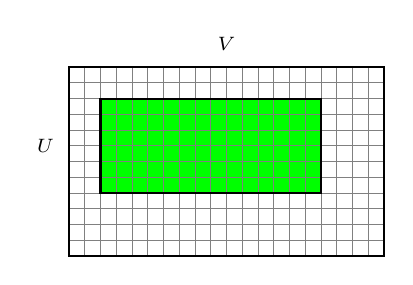
\begin{tikzpicture}
    \draw[fill = green] (0.4, -0.4) rectangle (3.2, -1.6);
    \draw[step = 0.2, gray, thin] (0, 0) grid (4, -2.4);
    \draw[black, thick] (0, 0) rectangle (4, -2.4);
    \draw[black, thick] (0.4, -0.4) rectangle (3.2, -1.6);
    \node at (-0.3, -1.) {\scriptsize $U$};
    \node at (2, 0.3) {\scriptsize $V$};
\end{tikzpicture}

            \end{center}
        \end{column}

		\begin{column}{0.48\textwidth}
            \begin{center}
                Треугольники:
                \vspace{0.2cm}
                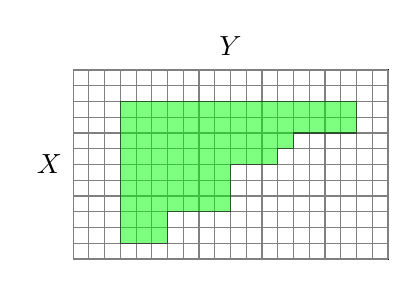
\begin{tikzpicture}
    \draw (0, 0) rectangle (4, -2.4);
    \draw[step = 0.2, gray, thin] (0, 0) grid (4, -2.4);
    
    \draw[fill = green, opacity = 0.5] (0.6, -0.4) -- (3.6, -0.4) -- (3.6, -0.8) -- (2.8, -0.8) -- (2.8, -1) --
    	(2.6, -1) -- (2.6, -1.2) -- (2, -1.2) -- (2, -1.8) -- (1.2, -1.8) -- (1.2, -2.2) -- (0.6, -2.2) --
        cycle;
    \node at (-0.3, -1.2) {$X$};
    \node at (2, 0.3) {$Y$};
\end{tikzpicture}

            \end{center}
		\end{column}
	\end{columns}
\end{frame}


\begin{frame}{$\KWm$ отношение (еще раз)}

    $f:\{0, 1\}^n \to \{0, 1\}$ монотонная частичная функция
    
    \begin{itemize}
        \item Алиса получает $x \in f^{-1}(1)$, Боб получает $y \in f^{-1}(0)$;
        \item цель~--- найти такую позицию $i \in [n]$, что $x_i = 1 \land y_i = 0$.
    \end{itemize}

    \pause

    \begin{theorem}[Разборов 95; Pudl{\'{a}}k 10; С 17]
        Для функции $f$ существует монотонная булева \alert{схема} размера $S$ тогда и только тогда, когда
        существует коммуникационный протокол \alert{на графе} для $\KWm_f$ размера $S$.
    \end{theorem}

    \pause

    \begin{theorem}[Hrube{\v{s}} Pudl{\'{a}}k 17]
        Для функции $f$ существует монотонная \textcolor{blue}{вещественная} схема размера $S$ тогда и
        только тогда, когда существует коммуникационный протокол с треугольниками на графе для $\KWm_f$
        размера $S$.
    \end{theorem}
\end{frame}


\begin{frame}{$\Search_{\varphi}$ (Lov{\'{a}}sz et al. 1994)}
    
    $\varphi(x, y)$~--- невыполнимая формула в КНФ:
    \begin{itemize}
        \item Алиса получает подстановку переменным $x$, Боб получает подстановку переменным $y$;
        \item цель~--- найти клоз $C \in \varphi$, который не выполнен подстановкой.
    \end{itemize}

    \pause

    \begin{theorem}[Kraj{\'{\i}}{\v{c}}ek 95; С 17]
        $CC_{\log(n)}$-доказательство формулы $\varphi$ размера $S$ $\Rightarrow$ протокол на графе
        размера $\poly(n) S$ для $\Search_{\varphi}$.
    \end{theorem}

    Резолюция, $\CP^*$, $\dots$~--- $CC_{\log(n)}$ системы доказательств.

    \pause
    
    \begin{theorem}[С 17]
        $\CP$-доказательство формулы $\varphi$ размера $S$ $\Rightarrow$ протокол с треугольниками на
        графе размера $S$ для $\Search_{\varphi}$.
    \end{theorem}
\end{frame}
  %  \begin{frame}{Граф решений. $S \subseteq \{0, 1\}^n \times \mathcal{T}$}
    $C(\rho) = \{z \in \{0, 1\}^n \mid z \sim \rho\}$
    
    \begin{columns}[t]
        \begin{column}{0.55\textwidth}
            \begin{itemize}
                \item $H$~--- граф с исходящей степенью $2$, $\forall h \in H, ~ {\rho}_h$~--- частичная
                    подстановка;
                \item $\rho_{root} = \emptyset$ ($C(\rho_{root}) \equiv 1$);
                \item если $a, b$ дети $h$, то $C(\rho_{h}) \subseteq C(\rho_a) \cup C(\rho_b)$;
                \item если $h$ лист, то $h$ помечен решением для $C(\rho_h)$.
            \end{itemize}
        \end{column}

		\begin{column}{0.4\textwidth}
            \begin{center}
                \tikzstyle{inner} = [thin, circle, minimum size = 0.4cm, draw, inner sep = 0.1pt, black, opacity = 1]
\tikzstyle{inner_g} = [thin, circle, minimum size = 0.4cm, draw, inner sep = 0.1pt, black, fill =
    green, opacity = 1]
\tikzstyle{ed} = [thick, ->, draw, black, opacity = 1]

    
\begin{tikzpicture}[>=stealth']
    \node[inner_g] (a) at (0, 0) {};
    \node[inner_g] (b) at (-0.9, -1.2) {};
    \node[inner] (c) at (0.9, -1.2) {\scriptsize $\rho_h$};
    \node[inner] (d) at (-1.5, -2.4) {\scriptsize $t_1$};
    \node[inner_g] (e) at (-0.3, -2.4) {\scriptsize $\rho_a$};
    \node[inner_g] (f) at (1, -2.4) {\scriptsize $\rho_b$};
    \node[inner_g] (g) at (-1.5, -4.3) {\scriptsize $t_2$};
    \node[inner] (h) at (-0.25, -4.3) {\scriptsize $t_3$};
    \node[inner_g] (g2) at (1.5, -4.3) {\scriptsize $t_3$};
    \node[inner] (h2) at (0.25, -4.3) {\scriptsize $t_2$};
    
    \path (a) edge[ed] (b);
    \path (a) edge[ed] (c);
    \path (b) edge[ed] (d);
    \path (b) edge[ed] (e);
    \path (c) edge[ed] (e);
    \path (c) edge[ed] (f);
    \path (e) edge[ed] (g);
    \path (e) edge[ed] (h);
    \path (f) edge[ed] (g2);
    \path (f) edge[ed] (h2);
\end{tikzpicture}

            \end{center}
		\end{column}
	\end{columns}

    Ширина графа решений: $\max\limits_{h \in H} |\rho_h|$.
\end{frame}

\begin{frame}{Result}
    \begin{itemize}
        \item $S \subseteq \{0, 1\}^n \times \mathcal{T}$;
        \item $w(S)$~--- минимальная ширина графа решений;
        \pause
        \item $\Ind: [m] \times \{0, 1\}^m \to \{0, 1\}$, где $m = n^{O(1)}$;
        \item $\Ind(x, y) = y_x$;
        \pause
        \item $S \circ \Ind$~--- коммуникационная задача поиска.
    \end{itemize}

    \only<1-3>{
    \onslide<3>{
        \begin{center}
              \begin{tikzpicture}
    \node[thick, circle, draw] (S) at (0, 0) {\Large $S$};
    
    \foreach \i in {1, 2, ..., 5}{
        \node (z\i) at (-3 + \i, -1.5) {$z_{\i}$};
        \draw[->] (z\i) -- (S);
    }
    
    \node[minimum height = 1cm, single arrow, draw] at (3, 0) {composition};

    \node[thick, circle, draw] (S1) at (6, 0) {\Large $S$};

    \foreach \i in {1, 2, ..., 5}{
        \node[draw, circle] (i\i) at (3 + \i, -1.5) {\scriptsize $g$};
        \draw[->] (i\i) -- (S1);

        \node (x\i) at (2.75 + \i, -2.4) {\scriptsize $x_{\i}$};
        \node (y\i) at (3.25 + \i, -2.4) {\scriptsize $y_{\i}$};
        \draw[->] (x\i) -- (i\i);
        \draw[->] (y\i) -- (i\i);
    }
\end{tikzpicture}
        \end{center}
    }}

    \only<4>{
        \vspace{0.86cm}
        \begin{theorem}
            Размер протокола на графах (с треугольниками) для $S \circ \Ind_m$ равен $n^{\Theta(w(S))}$.
        \end{theorem}
        \vspace{1.8cm}
    }
\end{frame}
   % \begin{frame}{Open problems}

    \begin{itemize}
        \item Better separations between $\OBDD(\land)$ and resolution.
        \item Lower bounds for $\OBDD(\land, \weakening, \reordering)$.
        \item A simulation of $\OBDD(\land, \weakening)$ by Frege?
    \end{itemize}
    
\end{frame}

   % \section{Part II: From Proofs to Computations}

    %\begin{frame}{Certificate of unsatisfiability}

    $\varphi(x, y) = \bigwedge\limits_{i = 1}^{m} C_i(x, y)$

    \vspace{0.5cm}

    $U_{\varphi}, V_{\varphi} \subseteq \{0, 1\}^m$:
    \begin{itemize}
        \item $A \in U_{\varphi} \Leftrightarrow \bigwedge\limits_{i \in A} C_i|_{x}$ is satisfiable;
        \item $A \in V_{\varphi} \Leftrightarrow \bigwedge\limits_{i \in A} C_i|_{y}$ is unsatisfiable.
    \end{itemize}

    $C_{x}$ ($C_{y}$) is a restriction of $C$ to the variables from $x$ ($y$) part.

    \begin{lemma}[Hrube{\v{s}}, Pudl{\'{a}}k 17 (implicit)]
        $\Search_{\varphi} \approx \KWm(U_{\varphi}, V_{\varphi})$.
    \end{lemma}
\end{frame}


\begin{frame}{Monotone span programs over field $\mathbb{F}$}

    \begin{tabular}{c|cccccccc}
        & & & & & & & &\\
        \hline
        $x_1$ & 0 & 2 & 3 & 1 & 0 & 2 & 1 & 0\\
        $x_3$ & 2 & 1 & 0 & 0 & 2 & 0 & 0 & 1\\
        $x_4$ & 1 & 0 & 0 & 0 & 0 & 0 & 0 & 0\\
        $x_5$ & 3 & 2 & 1 & 4 & 0 & 2 & 1 & 0\\
        $x_1$ & 0 & 2 & 3 & 1 & 3 & 2 & 4 & 0\\
    \end{tabular}

    \vspace{0.3cm}
    
	Is there $(1, 1, 1, \dots)$ in the span of selected vectors?

    \vspace{0.3cm}

	Size is a number of columns.
    
    \begin{lemma}[Pudl{\'{a}}k ??]
        $\forall f, mSP(f) \le mF(f)$.
    \end{lemma}

\end{frame}

\begin{frame}{Span programs and Nullstellensatz}

    \begin{lemma}[modification of Pudl{\'{a}}k, Sgall ??]
        $\NS$-proof of $\varphi(x, y)$ of $y$-degree $d$ $\Rightarrow$ $mSP(U_{\varphi}, V_{\varphi})$ of
        size $n^d$.
    \end{lemma}

    \pause

    \begin{lemma}[Pitassi, Robere 18]
        There is gadget $g$ such that $mSP(U_{\varphi \circ g}, V_{\varphi \circ g}) =
        n^{\Theta(\NS(\varphi))}$.
    \end{lemma}

    \pause

    \begin{lemma}
        $\NS$-proof of $\varphi$ of degree $d$ $\Rightarrow$ $\NS$-proof of $\varphi \circ \Ind_m$ of
        $y$-degree $d$.
    \end{lemma}

    $\Ind_m(x, y) = \sum\limits_{s \in [m]} \mathds{1}_{x = s} \cdot y_s$
\end{frame}


\begin{frame}{Separations}

    \begin{center}
        $\varphi$ is unsat CNF
	\end{center}

    \begin{minipage}{0.5 \textwidth}
        \centering
        Upper bound
    \end{minipage}%
    \begin{minipage}{0.5 \textwidth}
        \centering
        Lower bound
    \end{minipage}

    \pause
    \vspace{0.4cm}

    \begin{minipage}{0.5 \textwidth}
        \centering
        $\NS$-degree of $\varphi$
    \end{minipage}%
    \begin{minipage}{0.5 \textwidth}
        \centering
        resolution width of $\varphi$
    \end{minipage}

    \pause
    \vspace{0.3cm}

    \begin{minipage}{0.5 \textwidth}
        \centering
        $\Downarrow$ [PS]

        \vspace{0.3cm}

        $mSP(U_{\varphi \circ \Ind}, V_{\varphi \circ \Ind})$
    \end{minipage}%
    \begin{minipage}{0.5 \textwidth}
        \centering
        $\Downarrow$

        \vspace{0.3cm}
        
        $mRC(U_{\varphi \circ \Ind}, V_{\varphi \circ \Ind})$
    \end{minipage}


    \pause
    \vspace{1cm}
    Goal is to find any formula of small width that separates Nullstellensatz and resolution.

\end{frame}


\begin{frame}{$\EoL[k]$}
    
\end{frame}
    %\begin{frame}{Span programs and Nullstellensatz}

    \begin{lemma}[modification of Pudl{\'{a}}k, Sgall 98]
        $\NS$-proof of $\varphi(x, y)$ of $y$-degree $d$ $\Rightarrow$ $mSP(U_{\varphi}, V_{\varphi})$ of
        size $n^d$.
    \end{lemma}

    \pause

    \begin{lemma}[Pitassi, Robere 18]
        There is gadget $g$ such that $mSP(U_{\varphi \circ g}, V_{\varphi \circ g}) =
        n^{\Theta(\NS(\varphi))}$.
    \end{lemma}

    \pause

    \begin{lemma}
        $\NS$-proof of $\varphi$ of degree $d$ $\Rightarrow$ $\NS$-proof of $\varphi \circ \Ind_m$ of
        $y$-degree $d$.
    \end{lemma}

    $\Ind_m(x, y) = \sum\limits_{s \in [m]} \mathds{1}_{x = s} \cdot y_s$
\end{frame}


\begin{frame}{Separations}

    \begin{center}
        $\varphi$ is unsat CNF
	\end{center}

    \begin{minipage}{0.5 \textwidth}
        \centering
        Upper bound
    \end{minipage}%
    \begin{minipage}{0.5 \textwidth}
        \centering
        Lower bound
    \end{minipage}

    \pause
    \vspace{0.4cm}

    \begin{minipage}{0.5 \textwidth}
        \centering
        $\NS$-degree of $\varphi$
    \end{minipage}%
    \begin{minipage}{0.5 \textwidth}
        \centering
        resolution width of $\varphi$
    \end{minipage}

    \pause
    \vspace{0.3cm}

    \begin{minipage}{0.5 \textwidth}
        \centering
        $\Downarrow$ [PS]

        \vspace{0.3cm}

        $mSP(U_{\varphi \circ \Ind}, V_{\varphi \circ \Ind})$
    \end{minipage}%
    \begin{minipage}{0.5 \textwidth}
        \centering
        $\Downarrow$

        \vspace{0.3cm}
        
        $mRC(U_{\varphi \circ \Ind}, V_{\varphi \circ \Ind})$
    \end{minipage}


    \pause
    \vspace{1cm}
    Goal is to find any formula of small width that separates Nullstellensatz and Resolution.

\end{frame}
    %\begin{frame}{$\EoL[k]$}
    \begin{minipage}{0.5 \linewidth}
        \tikzstyle{undir} = [thick]
\tikzstyle{dir} = [thick, ->, bend left = 12]
\tikzstyle{ver} = [thick, ->, draw, circle]

\begin{tikzpicture}[black, >=stealth']

    \node[ver] (A) at (0, 0) {};
    \node[ver] (B) at (2, 2) {};
    \node[ver] (C) at (3, 0) {};
    \node[ver] (D) at (4, 1) {};
    \node[ver] (E) at (3.5, 3.5) {};
    \node[ver] (F) at (-0.5, 3) {};

    \only<1>{
        \draw[undir] (A) to (B);
        \draw[undir] (A) to (C);
        \draw[undir] (B) to (C);
        \draw[undir] (C) to (D);
        \draw[undir] (B) to (D);
        \draw[undir] (D) to (E);
        \draw[undir] (E) to (F);
        \draw[undir] (F) to (A);
        \draw[undir] (B) to (F);
    }
    
	\only<2->{
        \draw[dir] (A) to (B);
        \draw[dir] (A) to (C);
        \draw[dir] (B) to (C);
        \draw[dir] (C) to (D);
        \draw[dir] (B) to (D);
        \draw[dir] (D) to (E);
        \draw[dir] (E) to (F);
        \draw[dir] (F) to (A);
        \draw[dir] (B) to (F);

        \draw[dir] (B) to (A);
        \draw[dir] (C) to (A);
        \draw[dir] (C) to (B);
        \draw[dir] (D) to (C);
        \draw[dir] (D) to (B);
        \draw[dir] (E) to (D);
        \draw[dir] (F) to (E);
        \draw[dir] (A) to (F);
        \draw[dir] (F) to (B);
    }
\end{tikzpicture}

    \end{minipage}%
    \begin{minipage}{0.5 \linewidth}
        \pause
        \pause
        \begin{itemize}
            \item $v: ~ \sum\limits_{e \in E^{in}_v} x_{e} - \sum\limits_{e \in E^{out}_v} x_{e} = c(v)$
                \textcolor{red}{$(\mathbb{R})$};
            \item $\sum\limits_{v} c(v) = k$ \textcolor{red}{$(\mathbb{R})$};
            \item $k \neq 0 \Rightarrow \EoL[k]$ is unsat. 
        \end{itemize}
    \end{minipage}

    \pause
    \begin{lemma}
        $\EoL[1]$ has a low degree $\NS$-proof over any field.
    \end{lemma}
\end{frame}

\begin{frame}{Mystery of lines}

    \begin{lemma}[1]
        \begin{itemize}
            \item $\EoL[1]$ has a low degree $\NS$-proof over any field;
            \item $\forall k, \EoL[k]$ has a low degree $\NS$-proof over $\mathbb{R}$.
        \end{itemize}
    \end{lemma}

    \begin{lemma}[2]
        $G$ is $(n, d, \alpha)$-expander $\Rightarrow$ $w(\EoL[1]) = \Omega(n)$.
    \end{lemma}

    \begin{lemma}[3]
        $k = \mathrm{char}(\mathbb{F})^{\ell} \Rightarrow \exists G$, there is no $2^{\ell} =
        \Omega(\sqrt{n})$ degree $\NS$-proof of $\EoL[k]$ over $\mathbb{F}$.
    \end{lemma}

    \begin{itemize}
        \item $(1), (2) \Rightarrow$ separation between $mSP$ and monotone circuits;
        \item $(1), (3) \Rightarrow$ $mSP$ over $\mathbb{R}$ can be stronger than $mSP$ over fields with
            $\mathrm{char} > 0$. 
    \end{itemize}

\end{frame}


\begin{frame}{Open problems}

    \begin{enumerate}
        \item $k = \mathrm{char}(\mathbb{F})^{\ell}$. Can we prove $\Omega(n)$-degree lower bound?
        \item $k = \mathrm{char}(\mathbb{F})^{\ell}$. Polynomial calculus lower bounds?
        \item Model that can capture $mSP$ and monotone circuits simultaneously?
    \end{enumerate}
\end{frame}
\end{document}

